\documentclass[letterpaper]{article}

\usepackage{natbib,alifeconf}  %% The order is important
\usepackage{amsmath}
\usepackage{bbm}
\newcommand{\norm}[1]{\left\Vert #1\right\Vert}
\usepackage{url}

\usepackage{subcaption}
\graphicspath{{figures/}}
% *****************
%  Requirements:
% *****************
%
% - All pages sized consistently at 8.5 x 11 inches (US letter size).
% - PDF length <= 8 pages for full papers, <=2 pages for extended
%    abstracts.
% - Abstract length <= 250 words.
% - No visible crop marks.
% - Images at no greater than 300 dpi, scaled at 100%.
% - Embedded open type fonts only.
% - All layers flattened.
% - No attachments.
% - All desired links active in the files.

% Note that the PDF file must not exceed 5 MB if it is to be indexed
% by Google Scholar. Additional information about Google Scholar
% can be found here:
% http://www.google.com/intl/en/scholar/inclusion.html.


% If your system does not generate letter format documents by default,
% you can use the following workflow:
% latex example
% bibtex example
% latex example ; latex example
% dvips -o example.ps -t letterSize example.dvi
% ps2pdf example.ps example.pdf


% For pdflatex users:
% The alifeconf style file loads the "graphicx" package, and
% this may lead some users of pdflatex to experience problems.
% These can be fixed by editing the alifeconf.sty file to specify:
% \usepackage[pdftex]{graphicx}
%   instead of
% \usepackage{graphicx}.
% The PDF output generated by pdflatex should match the required
% specifications and obviously the dvips and ps2pdf steps become
% unnecessary.


% Note:  Some laser printers have a serious problem printing TeX
% output. The use of ps type I fonts should avoid this problem.


\title{Generating urban morphologies at large scales}
\author{Juste Raimbault$^{1,2,3,*}$ \and Julien Perret$^{1,4}$ \\
\mbox{}\\
$^1$UPS CNRS 3611 ISC-PIF\\
$^2$CASA, UCL\\
$^3$UMR CNRS 8504 G{\'e}ographie-cit{\'e}s\\
$^4$Univ. Paris-Est, LaSTIG STRUDEL, IGN, ENSG\\
\medskip
* juste.raimbault@polytechnique.edu} % email of corresponding author

% For several authors from the same institution use the same number to
% refer to one address.
%
% If the names do not fit well on one line use
%         Author 1, Author 2 ... \\ {\Large\bf Author n} ...\\ ...
%
% If the title and author information do not fit in the area
% allocated, place \setlength\titlebox{<new height>} after the
% \documentclass line where <new height> is 2.25in



\begin{document}
\maketitle

\begin{abstract}
% Abstract length should not exceed 250 words
  At large scales, typologies of urban form and corresponding generating processes remain an open question with important implications regarding urban planning policies and sustainability.
  We propose in this paper to generate urban configurations at large scales, typically of districts, with morphogenesis models, and compare these to real configurations according to morphological indicators.
  Real values are computed on a large sample of districts taken in European urban areas.
  We calibrate each model and show their complementarity to approach the variety of real urban configurations, paving the way to multi-model approaches of urban morphogenesis.
\end{abstract}


%%%%%%%%%%%%%%%%%%%%%
\section{Introduction}


The study of forms of the built environment, and more precisely of the urban environment, has been the subject of different disciplines such as architecture, urban planning, or geography, with different approaches corresponding to various scales and processes \citep{moudon1997urban,gauthier2006mapping,kropf2009aspects}.
Establishing typologies of urban morphologies, and understanding their link with underlying urban growth processes, is nowadays a crucial issue for sustainability as a large majority of the world population live in cities and energy consumption is closely related to urban form through e.g. mobility patterns and automobile dependance \citep{newman2000sustainable}.


Although there is neither a unified definition of urban form, nor unified generative models and quantitative indicators to measure it, several approaches are close to the spirit of artificial life and generative social science~\citep{bonabeau1997classical,epstein1999agent}.
Procedural modeling \citep{watson2008procedural} aims at generating realistic cities, but is mostly focused on the visual impression given and does not consider realistic generative processes.
It is furthermore developed largely at larger scales than the one of the district \citep{Parish:2001:PMC:383259.383292}.
Approaches linked to urban planning have focused on the spatial distribution of land-use, at multiple scales \citep{liu2017future}, and proposed cellular automata models for urban sprawl, generally at the scale of the metropolitan area \citep{herold2003spatiotemporal}.

% rq : should not cite too much - paper size limit
%\cite{merrell2010computer} internal building layouts generation
%\cite{horner2007multi} multi-scale - link with commuting - based on land-use

Urban form can furthermore be characterized considering different components of the urban system, such as building themselves as in several examples given before, but also for example transportation networks such as road networks \citep{ye2014quantitative}. To what extent these layers are complementary remains an open question, despite a few investigations coupling the two such as \cite{raimbault2018urban} suggesting indeed complementary dimensions. Regarding the geometrical properties of building layouts at the scale of a district, that we denote to simplify as urban form at a large scale, systematic characterizations and generative models remains rather rare. \cite{achibet2014model} for example describes a model of co-evolution of building layout and road network.



This paper proposes a first step towards a systematic understanding of generative models of the urban form, at a large scale.
The approach taken here is similar to the one taken by \cite{raimbault2018calibration}, which computes urban form indicators at a mesoscopic scale (metropolitan area) and calibrates a reaction-diffusion morphogenesis model.
We consider real urban configurations at the scale of the district (fixed spatial window of 500m), compute their morphological characteristics, and use these measures to calibrate different generative models of urban layouts at the same scale.
Our contribution is twofold: (i) we synthesize a set of indicators relevant at this scale, and compute them on a large sample of real urban configurations in European urban areas; (ii) we provide three different generative models complementary in the type of processes taken into account, and calibrate these models on the real morphological measures. We show therein the complementarity of the different processes to produce the variety of real urban forms considered.
This is to the best of our knowledge the first time several generative models at this scale are systematically compared on a large number of real configurations through quantitative measures.
% on drop le random ?
% nope mais on peut pas vraiment le considerer comme un generateur, disons un modèle nul
% ok, je vais ajuster le commentaire des figures

The rest of this article is structured as follows.
First, we present the methods used in our work, including the measures allowing the comparison of urban forms, the proposed generative models and the method used to retrieve real urban configurations.
The results of the proposed approach are then explained together with the tools used in the calibration of the models.
Finally, the results are discussed.

%%%%%%%%%%%%%%%%%%%%%
\section{Methods} \label{sec:methods}

The approach taken requires both a robust way to quantify urban forms, through indicators that can be understood as features in the sense of machine learning, and generative models.

\subsection{Quantifying urban forms}

The quantification of urban form is in itself covered by a vast literature.
Recent work have proposed to apply deep learning techniques directly on vector data, such as \cite{2017arXiv170902939M} does, for a worldwide classification of road networks. Such an approach avoids the question of isolating relevant features.
However, as we aim at calibrating generative models, our quantification will make more sense with interpretable measures.
%devrait on justifier pourquoi on a besoin de mesures interprétables ???
%. je pense, en reaction a la tendance deep learning etc ? (mais c'est peut etre pas pertinent en effet)
\cite{boeing2018measuring} proposes an extensive review of existing measures from a large extent of disciplines, their implications for planning and design, and the relation with urban complexity. \cite{webster1995urban} uses image processing techniques such as contrast or Fourier analysis, to extract synthetic descriptions of urban areas from satellite imaging. \cite{fumega2014identification} provide a typology of cities in relation with energy consumption in the perspective of climate change. \cite{rode2014cities} relate indicators of urban form with residential heat-energy demand. Other complexity-related approaches such as fractal dimensions have been introduced as for example by \cite{batty1987fractal}.



In practice, we use a variety of indicators capturing different aspects, each being detailed below. We consider the local urban space as a square grid of width $\sqrt{N}$ with cells $1 \leq i \leq N$, and an urban configuration is a binary function $s_i \in \{0;1\}$ on these cells. For the computation of indicators, we consider underlying complementary networks, the building network $B$ defined as nodes in centroids of occupied cells and links between two occupied direct neighbor cells (one cell unit of distance between centroids), and the free space network $\bar{B}$ defined similarly on empty cells. This raster representation is convenient as compatible with the various types of indicators and generators as described below. We will consider $\sqrt{N}=50$ in the following, and real windows of width $500m$.
%  justify the raster configuration (wouldnt be more logical to have vector generators at this scale ? discuss on "patches" : we do not care about even smaller details in buildings (as architects could do), but on the spatial distribution of free/occupied space at the granularity of patches. consistent with morpho indicators as they are computed, specifically for morpho math.

\subsubsection{Basic indicators}
% building area, density, moran, average distance, number of buildings (components), average building area
Simple descriptive indicators considered are (i) the total building density $A = \frac{1}{N}\cdot \sum_i s_i$; (ii) the number of buildings given by the number of connected components of $B$; (iii) the average building area, i.e. the average size of $B$ connected components; (iv) Moran index capturing spatial autocorrelation (see \cite{raimbault2018calibration} for its definition in a similar setting), with a simple inverse distance weight function; (v) average distance between non-empty points (which also captures a level of concentration).


\subsubsection{Network indicators}
% avg detour, average component area

We also use indicators computed with the underlying networks: the average detour computed in the free space network $\bar{B}$, computed by randomly sampling 50 pairs of points in a connected component of $\bar{B}$ and computing the ratio between the network distance and the euclidian distance $d_{\bar{B}}/d_E$. This measures captures in a way the sinuosity of streets from a mobility viewpoint. We also consider the average size of open connected areas as the average size of the connected components of $\bar{B}$.


\subsubsection{Mathematical morphology indicators}
% dilation steps, erosion steps
% closing / opening not included - would require profile = f(kernel size)

Finally, indicators inspired from the field of mathematical morphology \citep{serra1983image} have already been applied to the quantification of urban form as for example by \cite{pesaresi2003recognizing}. Mostly used in image processing, these techniques proceed to the convolution of the image with a filter for example to simplify some morphological detail, what can be interpreted as a kind of spatial smoothing. We use here an indicator based on erosion with a filter of smallest size, which here removes points which 4 closest neighbors are not also occupied. We consider the total number of steps to fully erode the image, which is linked to building size. Similarly, using the operation of dilation, which in the contrary occupies points with at least one occupied neighbor, we consider the total number of dilation steps to fully fill the grid. This captures the size of open spaces. We do not consider indicators linked to opening and closing operations, as these would require more complex filters and for example their behavior as a function of kernel size.


Combining these morphological indicators, we have a total number of 9 indicators that can be computed on any binary grid, and that we will use in the following to compare real grids with generated grids of the same size.





%\subsection{Real urban morphologies}
% osm buildings
% not needed as procedure for osm data is explained in results



\subsection{Generative models}

We detail now the generative model introduced. A null model is also considered, to ensure the relevance of the morphological measures and the adjustments on these. It consists in a random grid generator, where each cell is occupied if a random uniform number between 0 and 1 is below a density parameter $d_R$.

%%%%%%%%%%%%%%
\begin{figure}
    \centering
    \begin{subfigure}[b]{0.2\textwidth}
        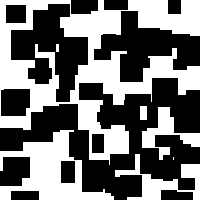
\includegraphics[width=\textwidth]{blocks}
        \caption{Blocks}
        \label{fig:blocks}
    \end{subfigure}
    \begin{subfigure}[b]{0.2\textwidth}
        
\includegraphics[width=\textwidth]{expMixture}
        \caption{Kernel mixture}
        \label{fig:mixture}
    \end{subfigure}
    \begin{subfigure}[b]{0.2\textwidth}
        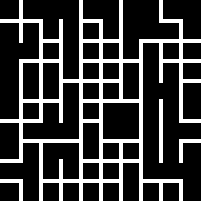
\includegraphics[width=\textwidth]{percolation}
        \caption{Network percolation}
        \label{fig:percolation}
    \end{subfigure}
    \begin{subfigure}[b]{0.2\textwidth}
        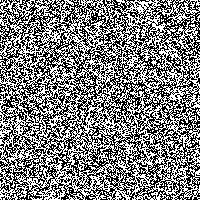
\includegraphics[width=\textwidth]{random}
        \caption{Random}
        \label{fig:random}
    \end{subfigure}
    \caption{Examples of patterns produced by the synthetic generators.}
    % TODO should provide parameters here
    \label{fig:generators}
\end{figure}
%%%%%%%%%%%%%%



\subsubsection{Blocks generator}

% bon, pour moi les deux premiers modèles sont des modèles procéduraux et pourraient êtres formalisés comme des mpp mais je ne sais pas si c'est pertinent de redire ça à chaque fois...
% -> d'accord avec toi !
The most simple ``realistic'' generator is similar to procedural modeling or marked point processes and distributes building blocks into the space (see Fig.~\ref{fig:blocks}). Given a number $N_B$ of blocks, random positions are drawn and block of a random height and width (with minimal value $m_B$ and maximal value $M_B$ as parameters) are placed at these.


\subsubsection{Kernel mixture generator}

Kernel mixture are a classical way to represent the spatial distribution of population density in an urban area \citep{anas1998urban} (see Fig.~\ref{fig:mixture}). They remain relevant at our scale, as they can be interpreted as a superposition of ``density hotspots'', as can the planning or the self-organization of a district can be. Given a number of centers $N_K$, $\vec{x}_{1\leq j \leq N_K}$ random position are drawn in the grid, at which kernels are applied, such that $s_i = \mathbbm{1}_{d_i \geq \theta_K}$ where the density $d_i$ for the point at position $\vec{y}_i$ is given by
\begin{equation}
    d_i = \frac{1}{N_K}\cdot \sum_j \exp{\left(-\norm{\vec{x}_j - \vec{y}_i}/d_K\right)} 
\end{equation}
where $d_K$ is a range parameter giving the extent of kernels.
% je ne suis pas convaincu par la formule : il y a un truc que j'ai raté ou il manque un vecteur
% si les x_i correspondent aux posistion des centres (hotspots), alors on ne calcule les densités que sur les hotspots et il nous manque la possibilité de calculer les densités pour les autres points. On aurait pas besoin de 2 vecteurs ? x_i => les centres, y_i => l'ensemble des points ?
% Dans le papier d'Anas il triche un peu : il utilise x_ij (mn dans le papier) pour la distance entre le point i et le centre j...
%. -> oui c'est ca, cetait pas les memes xi en effet cetait la coordone du point ou calculé ; renomme en yi comme tu suggerais

\subsubsection{Network percolation model}

The last generator we used is based on network percolation, in the spirit of capturing the constraints imposed by flows traversing a given urban area (see Fig.~\ref{fig:percolation}). While the two previous generator were based on building processes, this one relies on streets, and thus on processes linked to transportation. The idea is to link a fixed number $N_P$ of border points, which can be understood as entrances/exits of the area. Starting with a grid network without links and nodes at a regular spatial sampling (fixed with a step of 5 units in our case), an iterative procedure (i) draws a random number and add a random link at an empty potential link if it is smaller than a parameter called the percolation probability $p_P$; (ii) computes the largest connected component of the network and the number of nodes of this component on the boundary of the world; (iii) stops if this number is equal to the parameter $N_P$. Cells not covered by the resulting giant component are then occupied, at the exception of cells within a neighborhood $L_P$ of a link of the giant component. This way, this component can be understood as a circulating area linking $N_P$ entrances and exits, with a constraint on width through $L_P$.


Note that our generators will be ``fairly compared'' in terms of calibration, as they have the same number of parameters (although we do not introduce any information criteria that would yield the same penalization for overfitting).
We show in Fig.~\ref{fig:generators} visual representations of some outputs of each generator, including a random generator (see Fig.~\ref{fig:random}).


%%%%%%%%%%%%%%%%%%%%%
\section{Results} \label{sec:results}

Simulation results and real measures are available on the dataverse repository at \url{https://doi.org/10.7910/DVN/LGK0US}. Source code is available on the git repository of the project at \url{https://github.com/openmole/spatialdata}.
% TODO split repositories


%%%%%%%%%%%
\subsection{Real measures}

We compute the morphological indicators given above on a large sample on real urban areas. For practical computational reasons, we restrain our geographical area of study to European urban areas as provided by \cite{}. We expect to already have a good representativity, although not universal, of existing urban forms with this sample, as it is known that European cities already have a significant morphological diversity \citep{le2015forme}. We collect building layouts from OpenStreetMap (illustrated in Figure~\ref{fig:osm}), as this source has been shown to have a good quality especially in Europe \citep{mooney2010towards}. Using the \texttt{osmosis} tool, buildings are filtered from the openstreetmap raw dump for Europe (downloaded from \url{http://download.geofabrik.de/} in March 2019) and inserted into a Postgis database, which can then be efficiently queried for a specific bounding box. Indeed, although the library developed provides a direct access to the OpenStreetMap API, query limitations do not allow such a systematic sampling.
%Our tool also provide a direct access to the classic and overpass API % not necessary ?
We sample $N=72,000$ points into polygons corresponding to urban areas, first by selecting the area with a uniform selection weighted by population of areas, then by drawing uniform spatial coordinates within the polygon with a polygon sampling heuristic. % TODO clarify the polygon sampler

%  dim(real)
% 17612    16
%                           PC1    PC2     PC3
% Cumulative Proportion  0.7031 0.8592 0.92755

%%%%%%%%%%%%%%
\begin{figure}
    \centering
    \begin{subfigure}[b]{0.1\textwidth}
        \includegraphics[width=\textwidth]{{osm_(2.767548582324828,42.12774259047379)}.png}
    \end{subfigure}
    \begin{subfigure}[b]{0.1\textwidth}
        \includegraphics[width=\textwidth]{{osm_(2.956412030079216,48.95833438674378)}.png}
    \end{subfigure}
    \begin{subfigure}[b]{0.1\textwidth}
        \includegraphics[width=\textwidth]{{osm_(2.8534915107882908,48.87943398394085)}.png}
    \end{subfigure}
    \begin{subfigure}[b]{0.1\textwidth}
        \includegraphics[width=\textwidth]{{osm_(4.724576799597424,46.11247464316661)}.png}
    \end{subfigure}
    \begin{subfigure}[b]{0.1\textwidth}
        \includegraphics[width=\textwidth]{{osm_(6.693161940127149,51.28067900621835)}.png}
    \end{subfigure}
    \begin{subfigure}[b]{0.1\textwidth}
        \includegraphics[width=\textwidth]{{osm_(7.665417780766332,51.61719462734998)}.png}
    \end{subfigure}
    \begin{subfigure}[b]{0.1\textwidth}
        \includegraphics[width=\textwidth]{{osm_(7.746400123854242,49.448716515580514)}.png}
    \end{subfigure}
    \begin{subfigure}[b]{0.1\textwidth}
        \includegraphics[width=\textwidth]{{osm_(8.66720808445827,49.469125872820456)}.png}
    \end{subfigure}
    \begin{subfigure}[b]{0.1\textwidth}
        \includegraphics[width=\textwidth]{{osm_(8.368921085687871,49.224787816959754)}.png}
    \end{subfigure}
    \begin{subfigure}[b]{0.1\textwidth}
        \includegraphics[width=\textwidth]{{osm_(9.3988783289936,45.52643666558245)}.png}
    \end{subfigure}
    \begin{subfigure}[b]{0.1\textwidth}
        \includegraphics[width=\textwidth]{{osm_(9.422039749719488,48.68506062982569)}.png}
    \end{subfigure}
    \begin{subfigure}[b]{0.1\textwidth}
        \includegraphics[width=\textwidth]{{osm_(10.529303821177011,57.458935658684915)}.png}
    \end{subfigure}
    \caption{Samples extracted from OpenStreetMap.}
    % TODO should provide parameters here
    \label{fig:osm}
\end{figure}
%%%%%%%%%%%%%%

After removing the empty areas and areas with a too low (lower than 0.05) or a too high (higher than 0.8) density, we end with $17,612$ real points on which the morphological measures are computed. The effective dimension is relatively low, echoing literature on urban form at other scales, as the first principal component on normalized indicators captures 70.3\% of variance, the second a cumulated proportion of 85.9\% and the third 92.8\%. The order of magnitude are similar to the ones found by \cite{Schwarz201029} for example.

We obtain a broad variety of forms, measures such as the Moran index 

We can produce a typology of sampled urban areas through these measures.
% TODO typology of urban areas ?


% figure not needed : existence of clear distinctions (diversity index) and correlation with coordinates is enough
%%%%%%%%%%%%%%
%\begin{figure}
%    \centering
%    \includegraphics{}
%    \caption{Typology of morphological profiles of European urban areas.}
%    \label{fig:realtypology}
%\end{figure}
%%%%%%%%%%%%%%




%%%%%%%%%%%
\subsection{Direct sampling}

A first simulation experiment provides an insight into the patterns produced by the different generators in the morphological space. We sample the parameter space using a Latin Hypercube Sampling, with 10000 points for each generator respectively, and with 100 stochastic repetitions for each parameter point. The corresponding point cloud is shown in a reduced dimension in Fig.~\ref{fig:lhs}.
Regarding the stochastic variability of generators, % TODO sharpe ratios



%%%%%%%%%%%%%%
\begin{figure*}
    \centering
    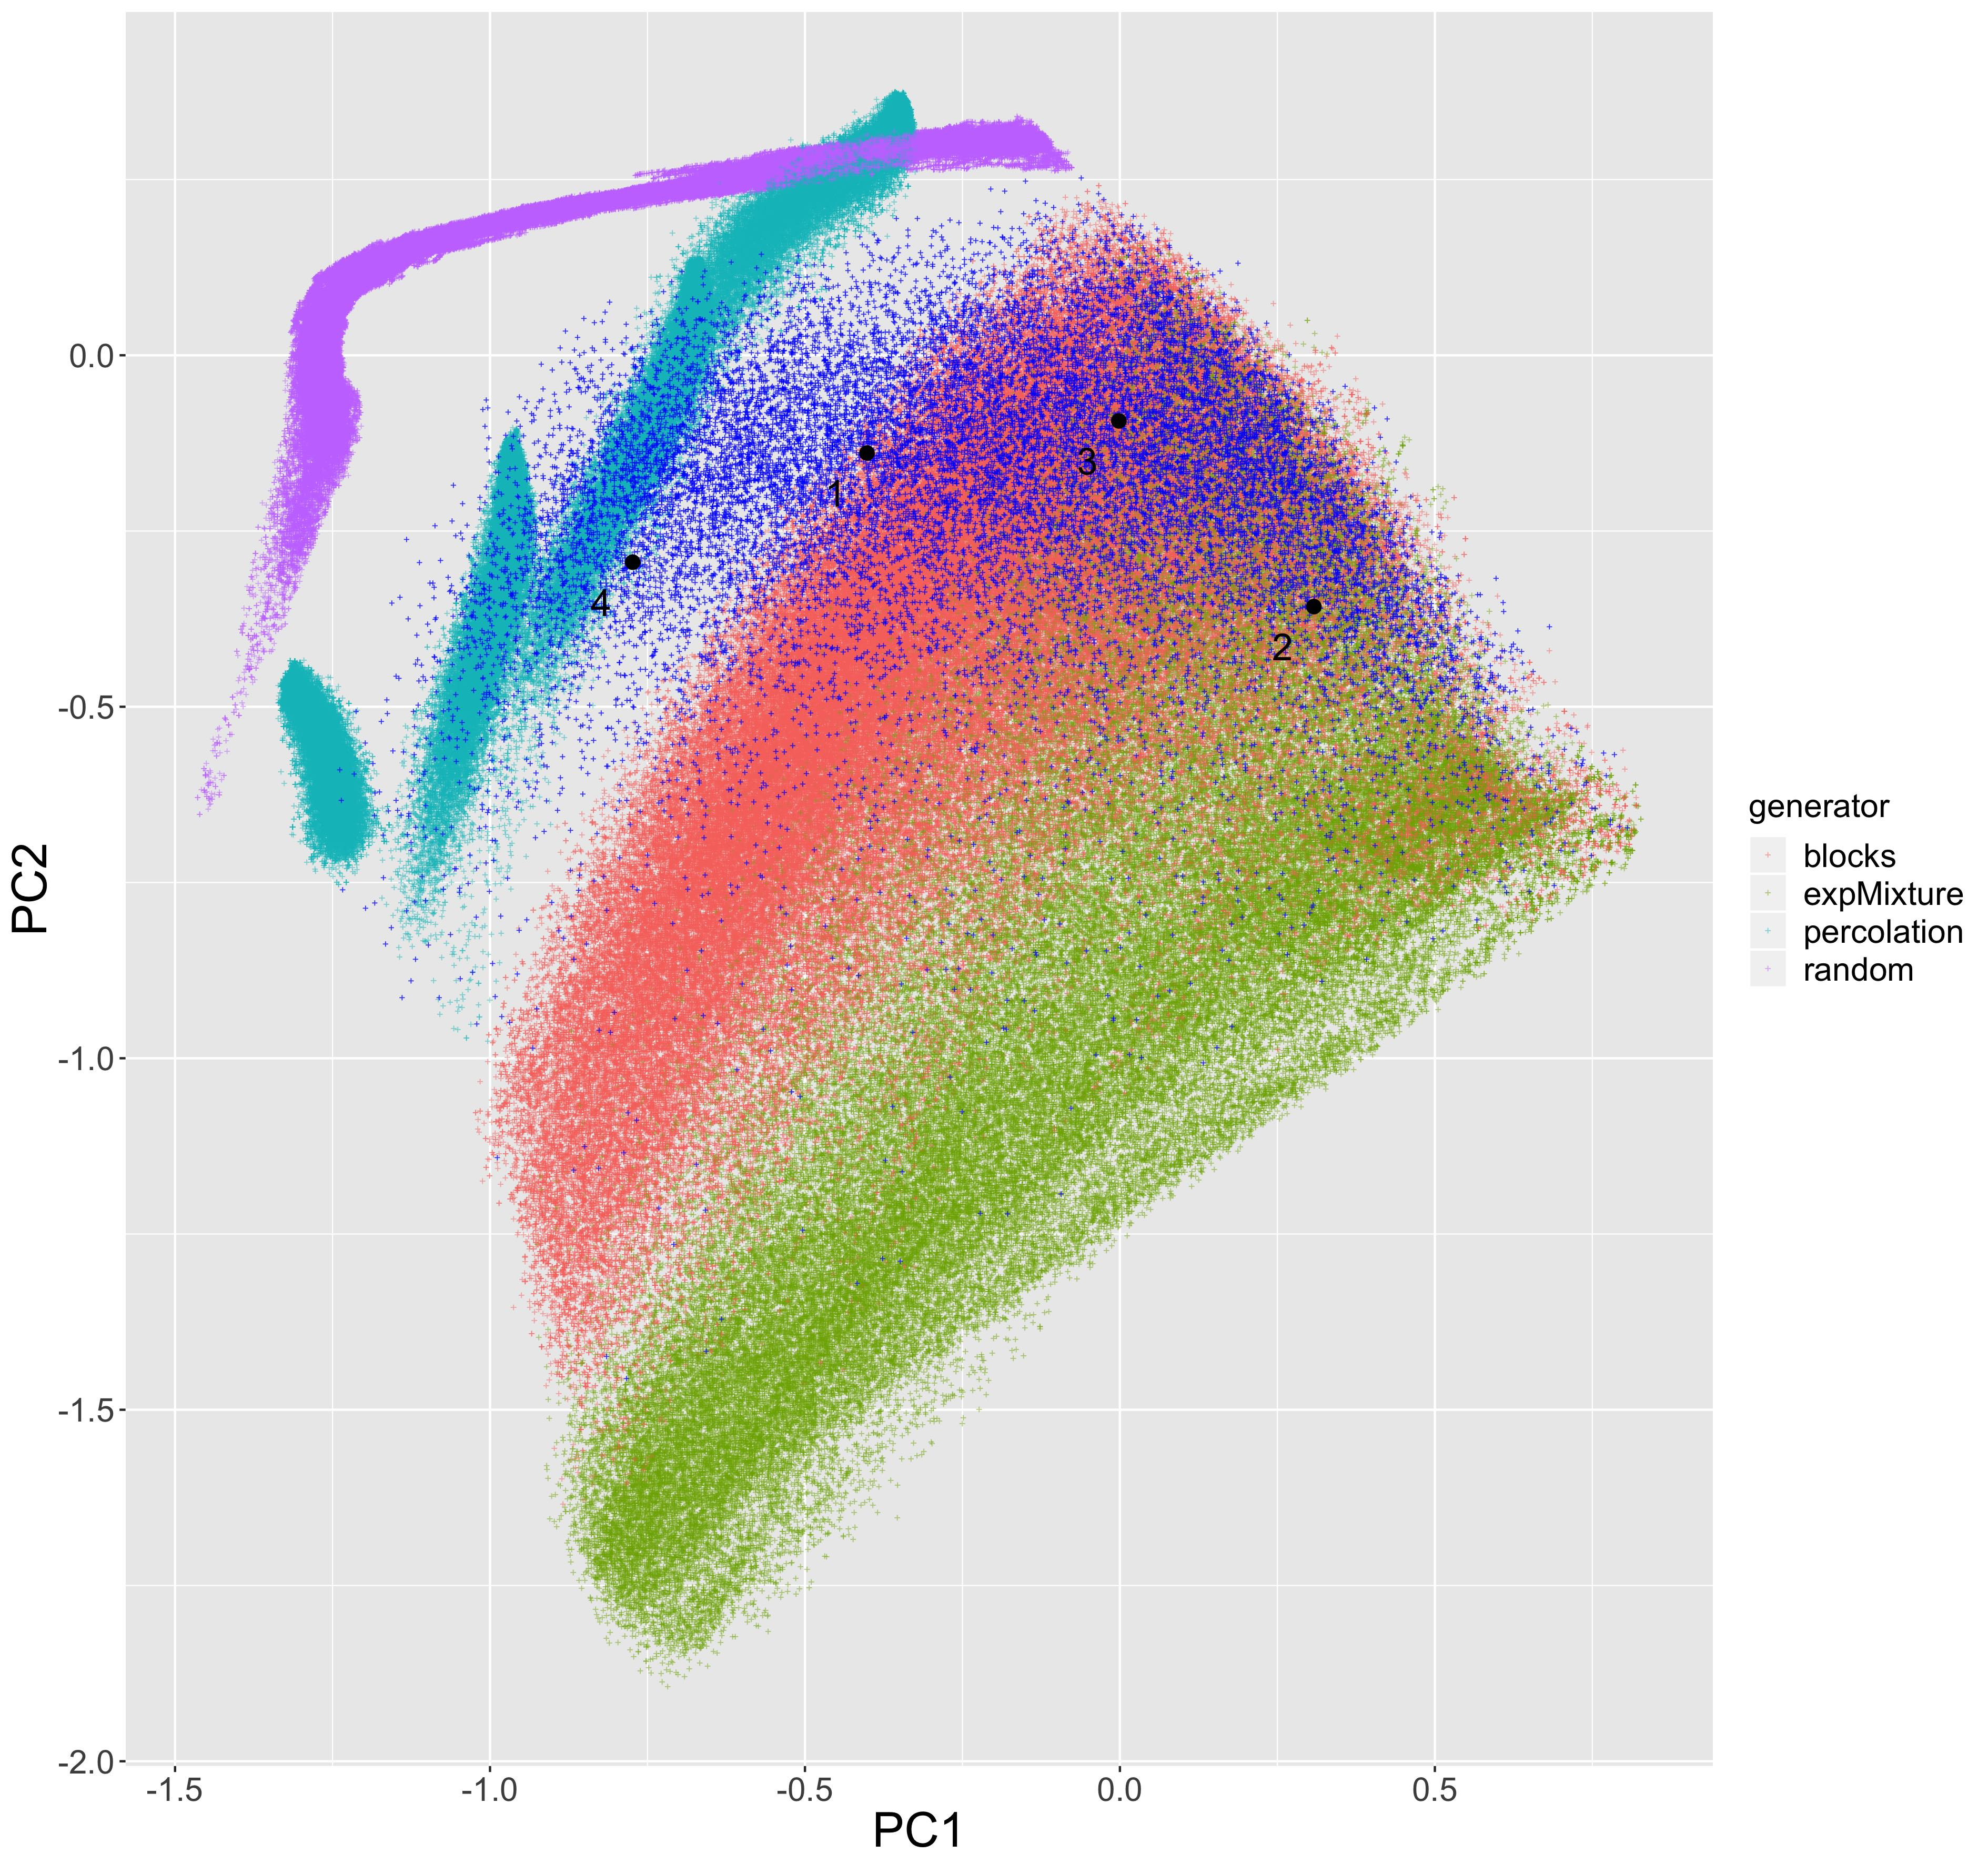
\includegraphics[width=\linewidth]{lhscalib_projrealpcs}
    % TODO figure a refaire + corresponding examples of morphologies
    \caption{Comparison of real morphologies with patterns produced by the synthetic generators. All points are projected into the first two components computed on the real measures only. Points in dark blue correspond to real configurations. The type of generator is given by the color in legend. Dark circle correspond to the centroids of clusters on which the calibration is done.}
    \label{fig:lhs}
\end{figure*}
%%%%%%%%%%%%%%



% les calibrations sont ULTRA mediocres, j'arrive pas a savoir pourquoi - pourtant ya beaucoup de runs - peut etre les islands trop courtes. on va surement devoir s'en resumer a un tableau de la distance de chaque generateur a chaque centroide ; avec l'info de plus de l'aggregation eventuellement - avec la sd.
%%%%%%%%%%%
%\subsection{Calibration with Genetic algorithms}
%The mapping between generator parameters and the morphological space being highly non-linear, we are not ensured that the proximities observed above fully correspond to the potentialities of generators to generate real forms. Therefore, we proceed here to a calibration of these models.



%%%%%%%%%%%%%%%%%%%%%
\section{Discussion} \label{sec:discussion}

% TODO if no credible calib results -> discuss how it could be done. Rq : the calibration in high dimension with a projection is tricky / not much studied -- cf similar issue with diversity algorithms and the proposal of a PSE-PCA.

Our approach provides a first step towards systematic modeling of generative processes of urban form at large scales, and can thus be extended in several ways.
First of all, we focused on the built environment but neglected transportation infrastructures, whereas spatial network morphogenesis models have been proposed for example by \cite{courtat2011mathematics} or \cite{raimbault2018multi} in a multi-modeling approach.
Taking into account multiple dimensions of the urban system is an important extension and hybrid models such as co-evolution models \citep{raimbault2014hybrid} should be investigated.

Furthermore, we tested the complementarity of generators only in a static way. Adaptive and dynamic generators, combining processes of different nature within the same model with an endogenous switching or combination, would be an important direction to better understand urban morphogenesis.
In the same context, the generators compared here had all the same number of parameters, but richer generators implying different numbers would require the use of information criterions to avoid overfitting, what however remains an unsolved issue for such generative simulation models \citep{piou2009proposing}.

Finally, as extensively reviewed above, the way to quantify urban form strongly depends on the scale considered. A more integrative understanding of it would require multi-scale approaches able to relate these different definition and measures within a single multi-scalar framework.





%%%%%%%%%%%%%%%%%%%%%
%\section{Conclusion}



%%%%%%%%%%%%%%%%%%%%%
\section{Acknowledgements}

Results obtained in this paper were computed on the vo.complex-system.eu virtual organization of the European Grid Infrastructure ( http://www.egi.eu ). We thank the European Grid Infrastructure and its supporting National Grid Initiatives (France-Grilles in particular) for providing the technical support and infrastructure.

\footnotesize
\bibliographystyle{apalike}
\bibliography{biblio} % replace by the name of your .bib file


\end{document}



%%%%%%%
%% Templates

%\begin{figure}[t] % [!tbp] % [ht]
%\begin{center}
%\includegraphics[width=2.2in, angle=90]{fig5.eps}
%\vskip 0.25cm
%\caption{Fitted exponent of power law for 34 runs at mutation rates  between $R=0.0005$ and $R=0.01$ copy errors per instruction  copied. The error bars reflect the standard deviation across the  sample of runs taken at each mutation rate. The solid line is to  guide the eye only.}
%\label{fig5}
%\end{center}
%\end{figure}


%\begin{table}[h]
%\center{
%\begin{tabular}{|c|c|c|c|}\hline
%Name & Result & Bonus $b_i$ & Difficulty\\ \hline\hline
%Echo & I/O   & 1 & --\\
%Xor  & $ A\ {\rm xor}\ B$ &   6 & 4 \\
%Equals &$\neg(A\ {\rm xor}\ B)$&6& 4 \\ \hline
%\end{tabular}
%}
%\vskip 0.25cm
%\caption{Logical calculations on random inputs $A$ and $B$ rewarded,bonuses, and difficulty (in minimum number of {\tt nand} instructionsrequired). Bonuses $b_i$ increase the speed of a CPU by a factor
%$\nu_i=1+2^{b_i-3}$.}
%\end{table}


